\section{The State Redistribution Algorithm}\label{sec:srdAlg}

In this section we describe only the second order accurate version of the State
Redistribution Algorithm. 
This helps simplify the notation and make the
algorithm more intuitive.   
At several places there are choices
to make, and we discuss the alternatives and the reason behind our
choices.  Since the postprocessing step comes after the finite
volume update step, we begin this section by briefly reviewing the 
two methods that SRD is applied to.  

\subsection{The Base  Finite Volume Schemes}

Our computational results will use two different finite volume schemes
to update the Cartesian cut cell mesh.
We will refer to these at the base schemes. 
The  update is applied to the entire mesh, including  
to the small cut cells.  Since cut cells can have cell volumes that are
orders of magnitude smaller than the time step allowed by the full
cells, these will lead to instability without a stabilization algorithm.
SRD will be applied after each stage or step of the base scheme.

\begin{figure}
\begin{center}
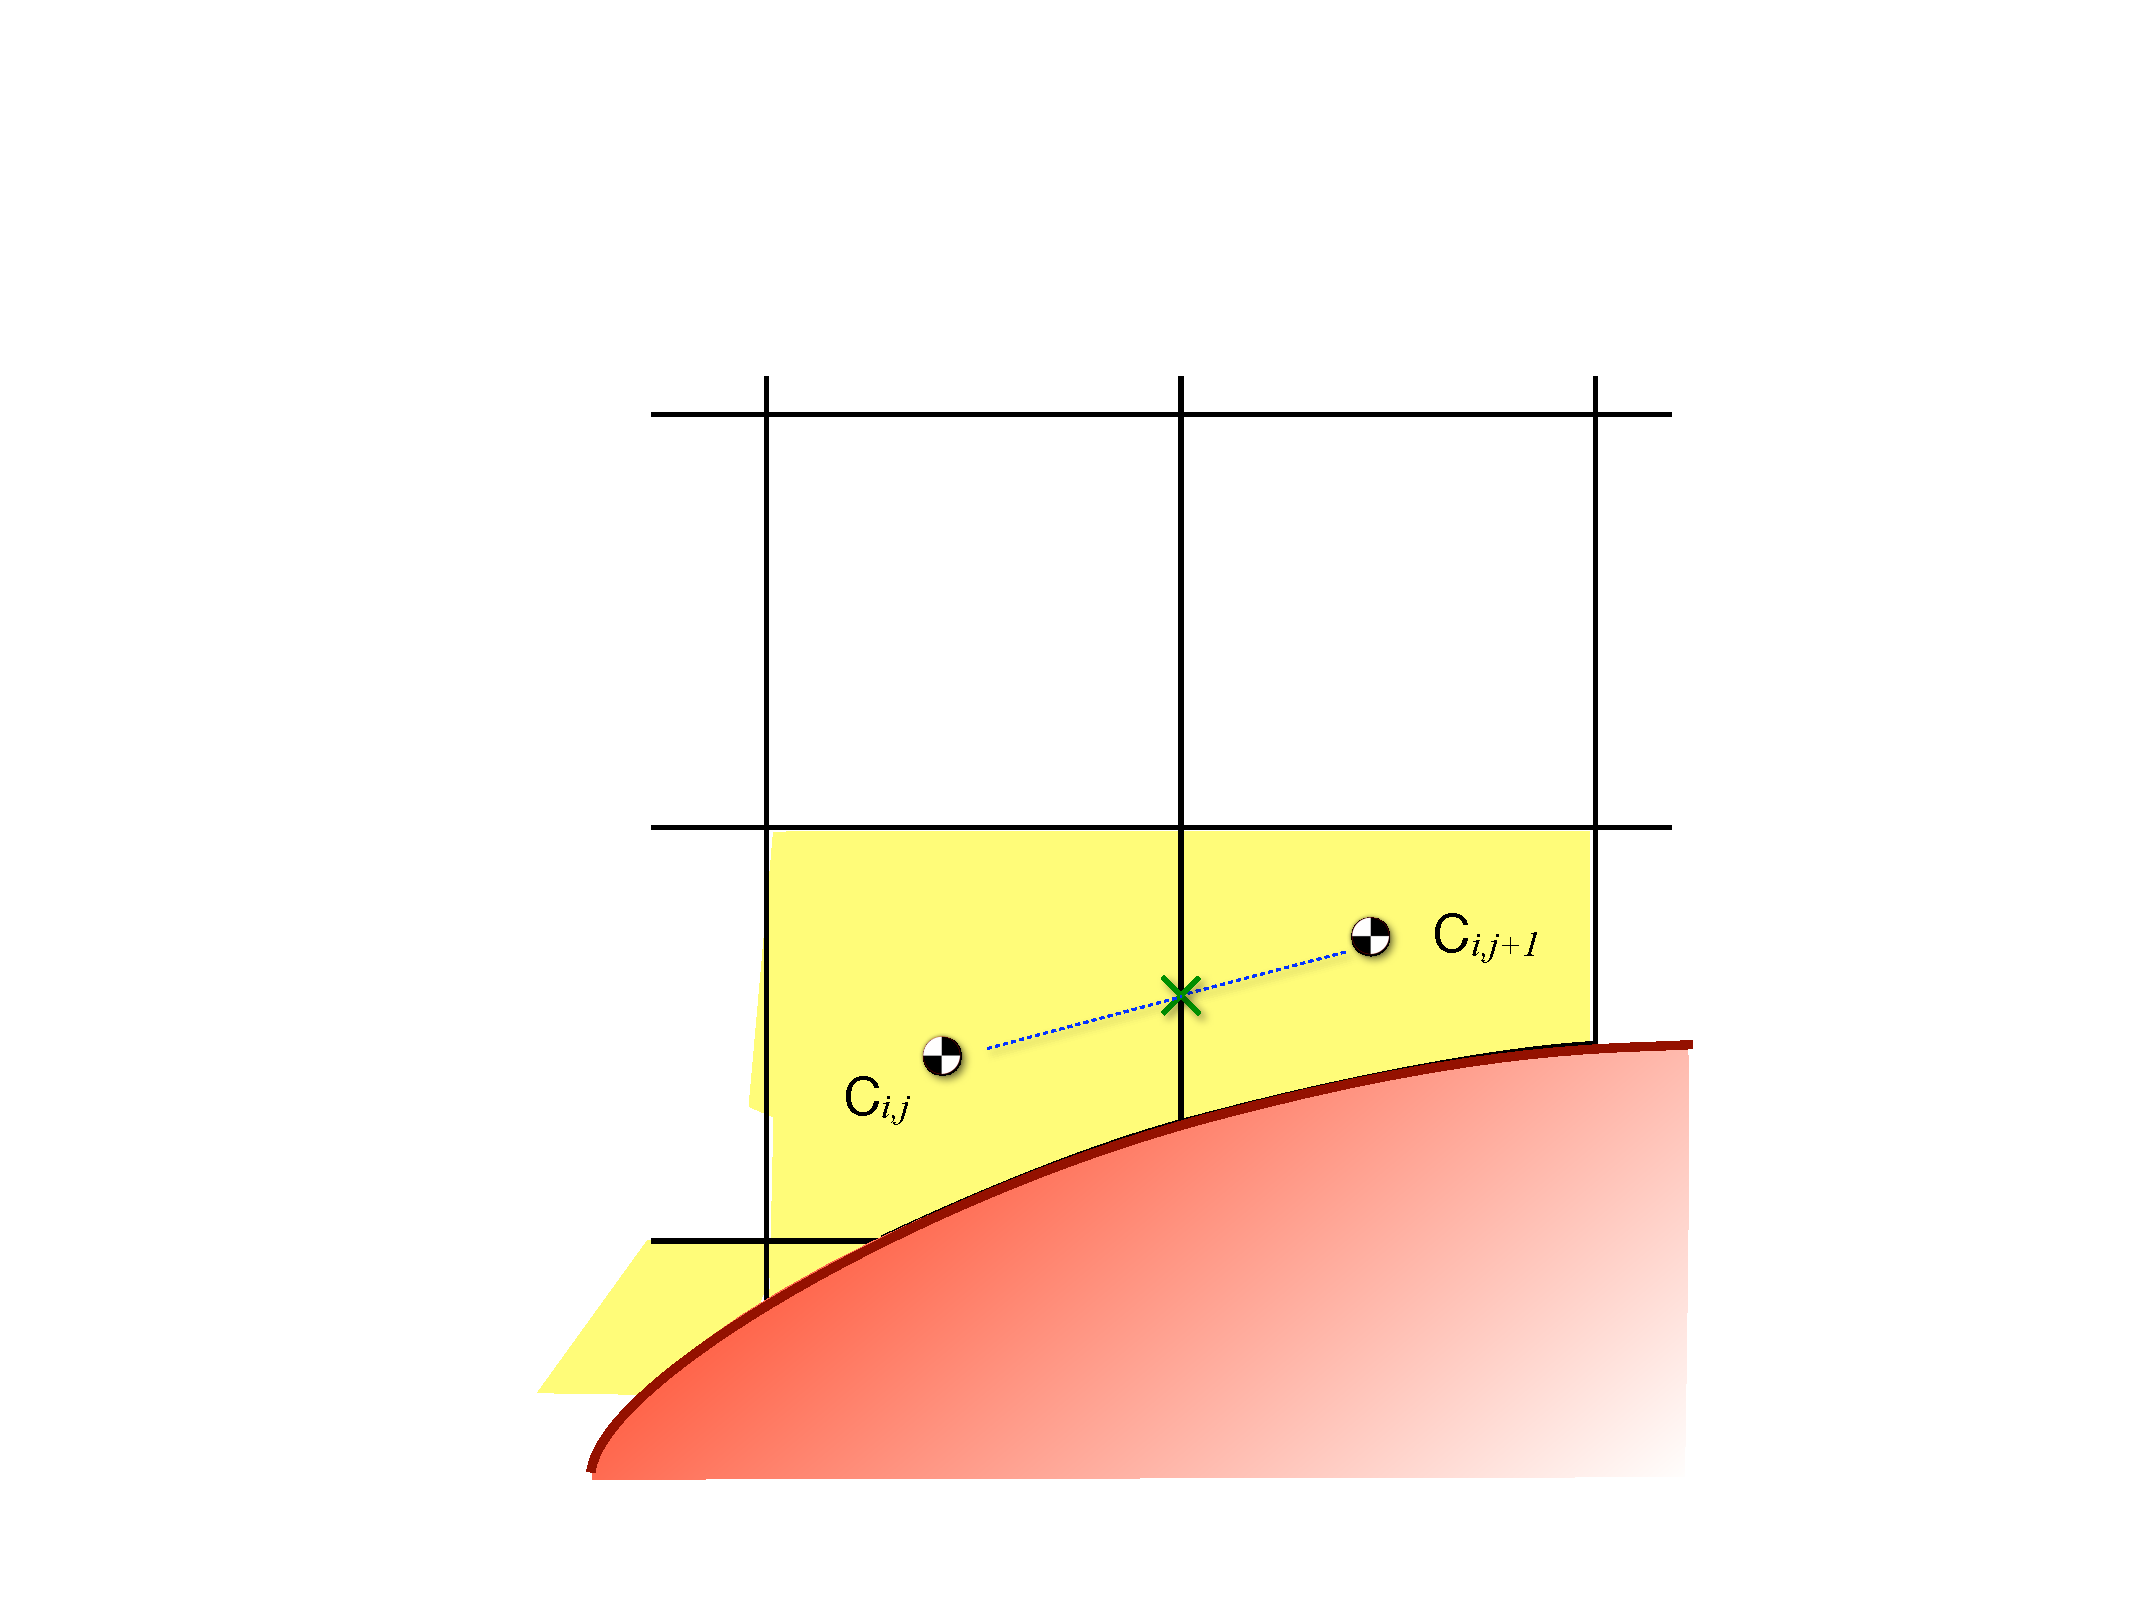
\includegraphics[width=2.8in]{figs/2dfig.pdf}
\caption{\sf Notation for mesh in two space dimensions. The cells shaded
in yellow are the cut cells.} 
\label{fig:2dfig}
\end{center}
\end{figure}

\subsubsection{Method of Lines approach}
The simplest scheme is to use a spatial discretization over the entire
mesh, and apply a Runge-Kutta scheme in time. This is a well-known
standard approach
on regular Cartesian meshes. It is adapted for the cut cells by
using a least squares reconstruction of the gradient that includes
either edge and node neighbors (unless otherwise specified).
Limiting is done using the Barth-Jespersen limiter \cite{} 
on the cut cells and one adjacent neighbors. Any limiter
can be used for the regular cells.

The spatial reconstruction in the cut cells is no longer
coordinate-aligned, and is modified
to include both $x$ and $y$ components of the gradient to 
reconstruct to the midpoint of the cell edge. This is indicated 
in figure \ref{fig:2dfig}  with a green `x'.
The SRD stabilization scheme is applied after each stage of
the Runge-Kutta scheme. 
Note that for stability, the TVD limit for the Euler equations using
this scheme is  (AG -
TRUE?)
\begin{equation}
\Delta t \,  \max\{\frac{u+c}{hx},\frac{v+c}{hy}\} < 0.5 
\end{equation}


\subsubsection{MUSCL scheme}
The MUSCL scheme is a one step method that is second order accurate in
time. The series of MUSCL schemes  was originated by van Leer 
\cite{vanleer:muscl}. The version we use 
is due to Colella \cite{Colella:Unsplit}.\footnote{Thanks to Phil 
Colella for the original Cartesian mesh code as well}.
We adapted it to cut cells by turning off the corner coupling 
This is the term that brings in the transverse derivatives. For example,
when computing the flux $f_{i+1/2,j}$ at time $t_{n+1/2}$, the 
term $ 1/2 \, \Delta t/\Delta y \, \partial G / \partial y$
appears.
(SAY MORE OR LEAVE WITH JUST REFERENCE)
On a regular mesh in  two space dimensions this term allows a
full stable timestep of 
\begin{equation}
\Delta t \,  \max\{\frac{u+c}{hx},\frac{v+c}{hy}\} < 1
\end{equation}
Without these terms the time step is reduced to 
\begin{equation}
\Delta t \, \left (\frac{u+c}{hx} + \frac{v+c}{hy} \right) < 1
\end{equation}
which could be as small as half the larger limit.
However, as shown in \cite{mjb:stability2} for one space dimension, 
boundary cells can have
a local {\em cfl} number that is up to twice the stable {\em cfl} of the regular
mesh and the overall scheme remains stable. So we are not concerned
about dropping this term only in the cut cells, and have observed no
stability problems. This does affect the accuracy in the cut cells
though. 

We also modified the prediction of the interface values to reconstruct
to the midpoint of the cell edges, and
modified the gradient in the cut cells to use a least squares routine.
ACCURACY OF THIS?
Other adaptations of MUSCL for cut cells are certainly possible and
worth investigating, but that is not the focus of this work.


\subsection{The State Redistribution Algorithm}

We first define two quantities associated with each cell of the mesh:

\begin{itemize}
\item
{\bf Each cut cell finds adjacent cells to {\em temporarily} merge with.}

\vspace*{.1in}
For each cut cell in the mesh, find  one or more neighbors until the
volume of the temporarily merged cell, $V_{\text{merge}}$, is at least half the area of an uncut cell, i.e., 
\begin{equation} \label{eq:vmerge}
V_{\text{merge}} \geq \frac{1}{2}\Delta x\Delta y.
\end{equation}
We call this the 
{\em  merging neighborhood} or {\em merging tile}.  
A small cell can be merged with cells in the direction closest to the boundary normal (Figure \ref{fig:neighborhoods}, left), or with all cells that are at most e.g. one cell away, that is, cells located on the $3 \times 3$ tile centered at the small cell (Figure \ref{fig:neighborhoods}, right).
The larger the neighborhood the more diffusive the results, therefore we use the normal neighborhood everywhere possible.
There are instances where the normal neighborhood cannot be used, e.g., if a neighboring cell is also cut and the
merging neighborhood is not sufficiently large (Figure \ref{fig:normalneighborhood}).  In this case, we must merge with cells on the $3\times3$ tile (Figure \ref{fig:3x3neighborhood}), or, if that merging neighborhood is not large enough, with cells on the $5 \times 5$ tile.

\begin{figure}
    \centering
    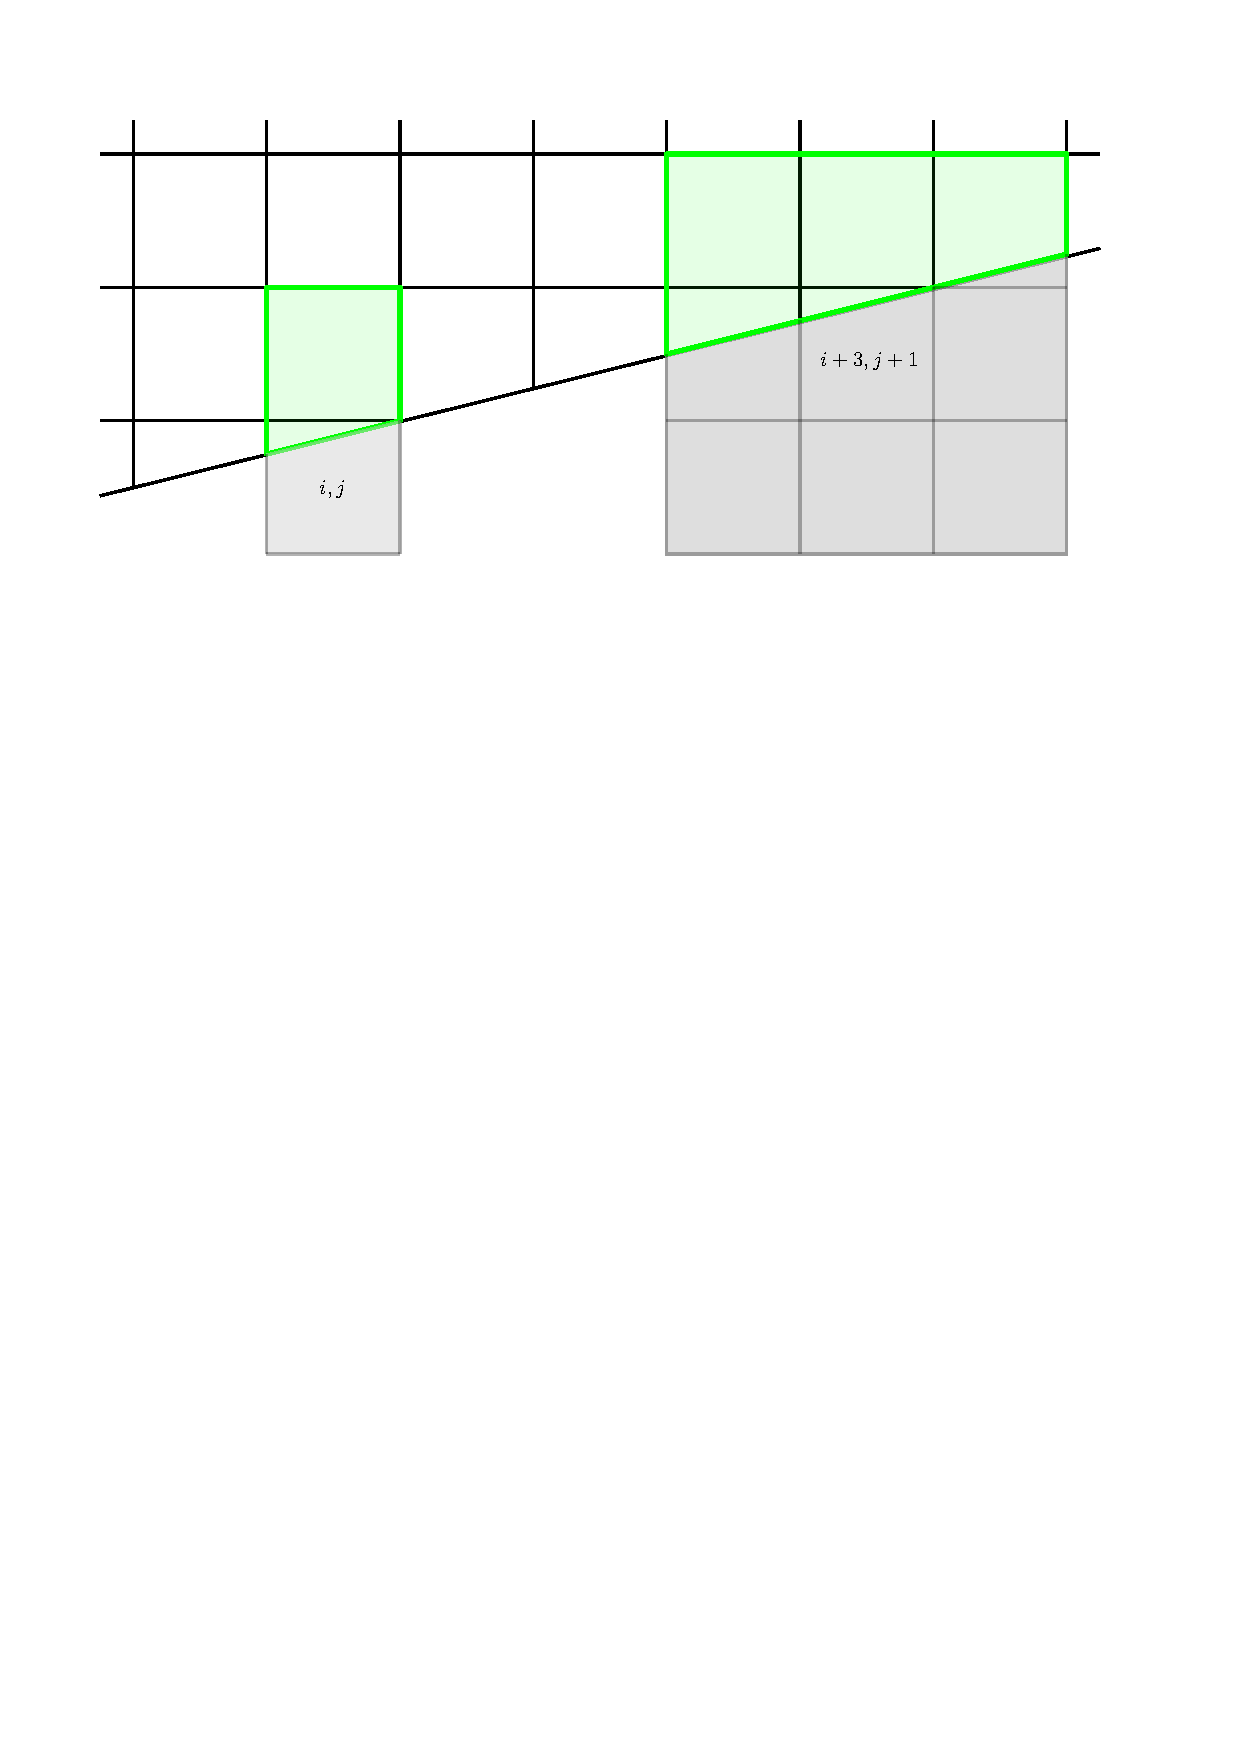
\includegraphics[width=0.5\linewidth]{figs/neighborhoods.pdf}
    \caption{On the left, a small cell is merged with a cell in the direction normal the wall.  On the right, a small cell is merged with neighbors that are at most one cell away, i.e., cells located on the $3\times3$ tile.}
    \label{fig:neighborhoods}
\end{figure}

\begin{figure}
	\subfloat[Normal neighborhood (in red) for both small cells.]{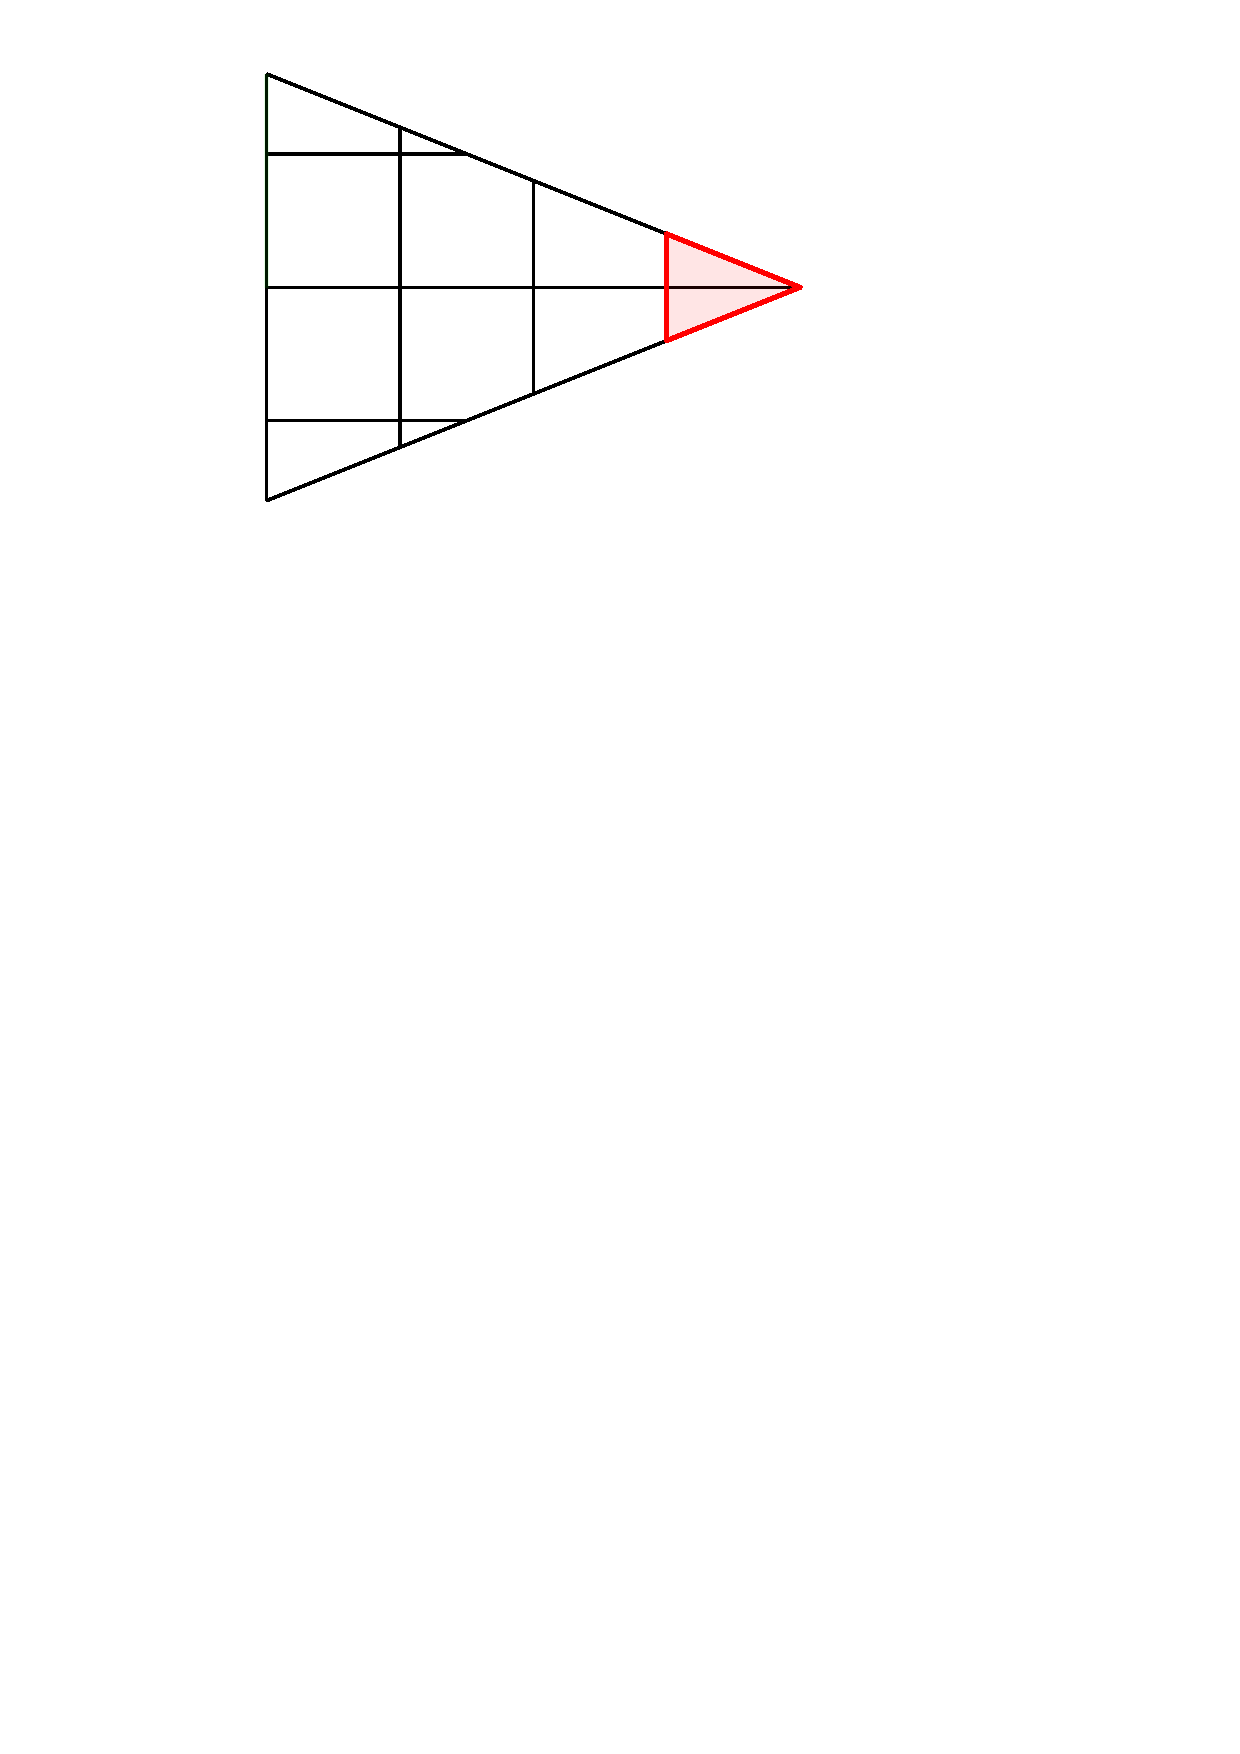
\includegraphics[width=.45\textwidth]{figs/normaldirection1.pdf} \label{fig:normalneighborhood}}
	\hfill
	\subfloat[$3\times 3$ merging neighborhood for both small cells.]{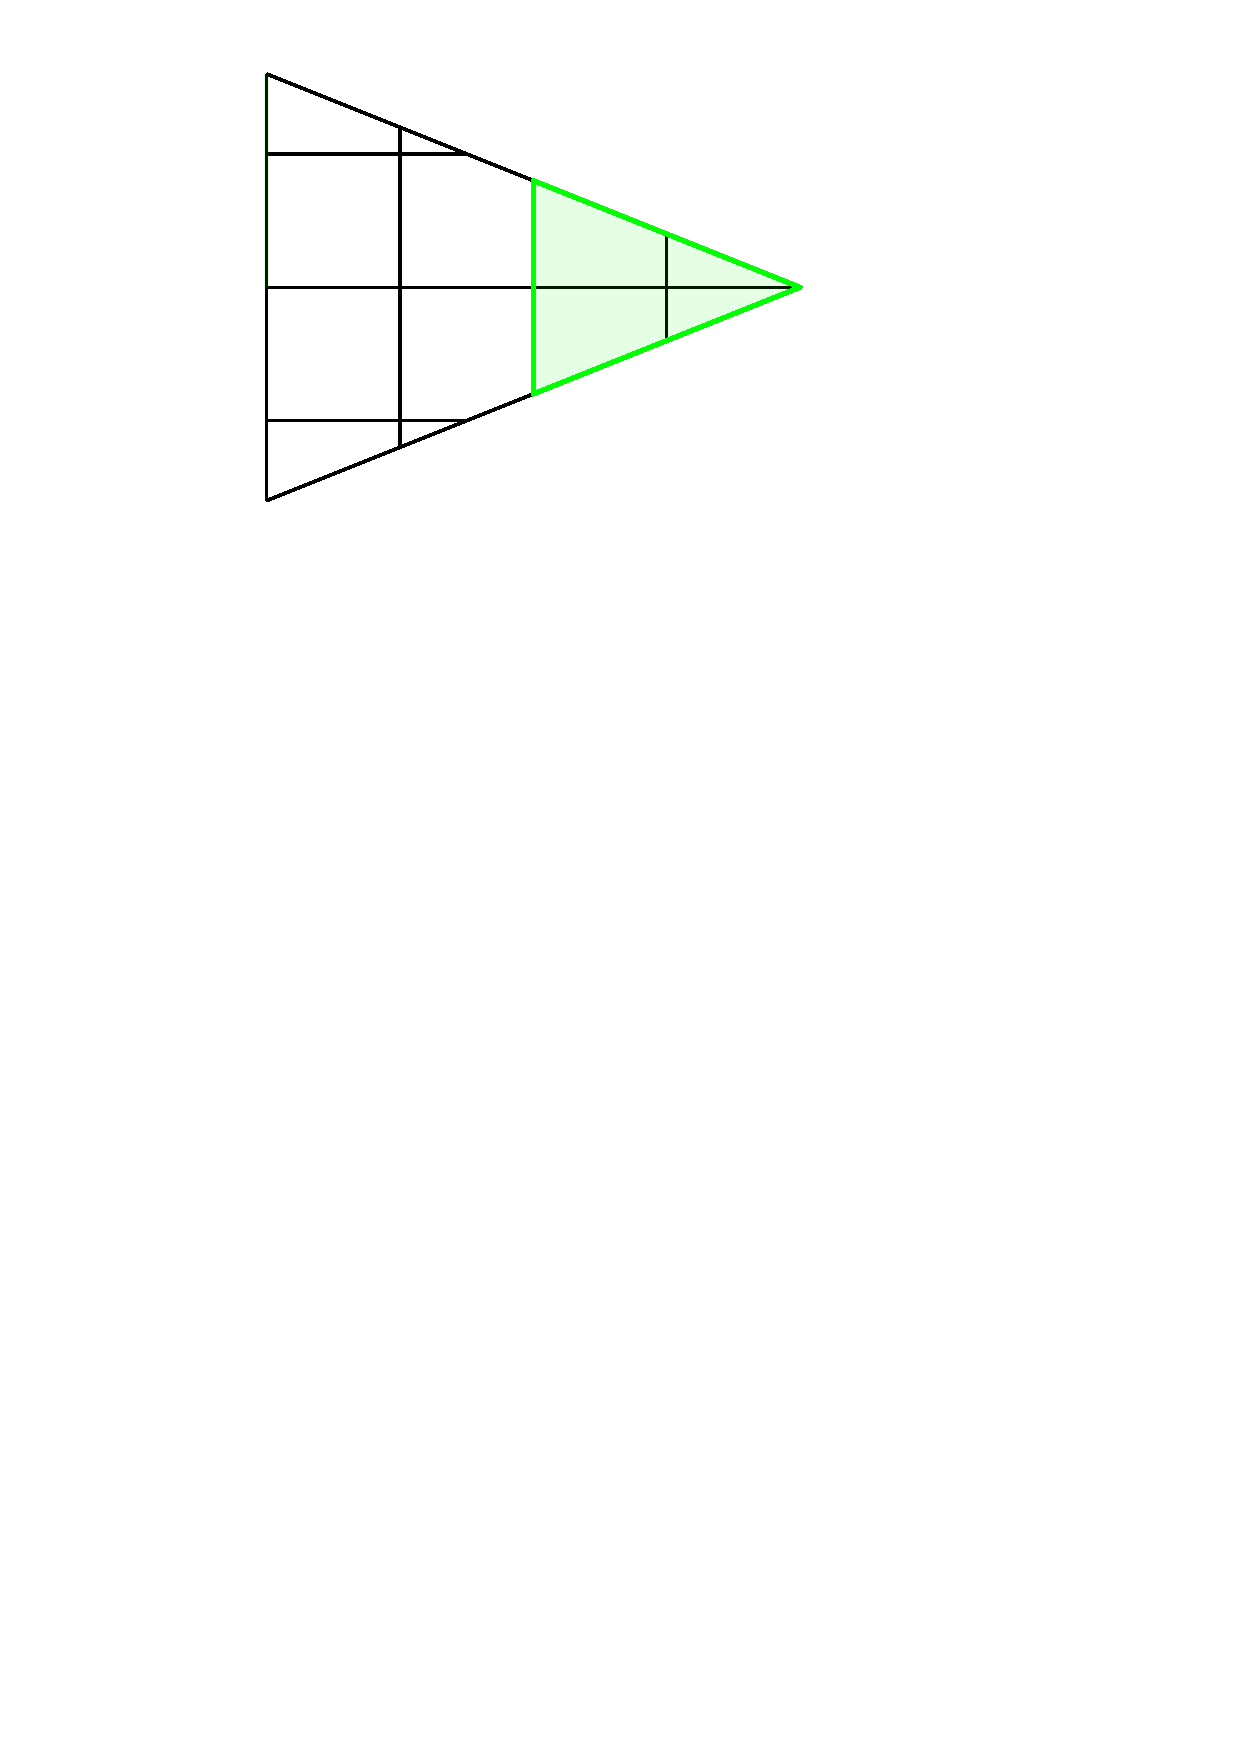
\includegraphics[width=.45\textwidth]{figs/normaldirection2.pdf} \label{fig:3x3neighborhood}}
	\caption{Sometimes, the normal neighborhood is not large enough if a small cell merges with another small cell.  In this case, we use the $3\times 3$ tile, or $5\times5$ neighborhood until the volume constraint \eqref{eq:vmerge} is satisfied.}
\end{figure}
% If the neighboring cell 
% is also cut, it can happen that the
% merged cell is not sufficiently large (SHOW EXAMPLE?). 
% Next we try a 2 by 2
% neighborhood, including the original cut cell. Later we also show
% results using a 3 by 3 neighborhoods. However the larger the
% neighborhood the more diffusive the results.

% Note that this does not have the difficulty of cell merging, since 
% overlapping neighborhoods are allowed. 

\item
{\bf Each cell counts how many neighborhoods it is a part of.}

\vspace*{.1in}
A full cell is its own merging neighborhood, since it has sufficient
volume all by itself. However, we will still refer to all cells as having a
merging neighborhood for ease of presentation.  In figure \ref{fig:overlappingneighs}, we provide an example cut cell mesh with all merging neighborhoods plotted.  We also display the number of overlapping neighborhoods on a cell, this is the neighborhood {\em count} for each cell.
\begin{figure}
	\subfloat[]{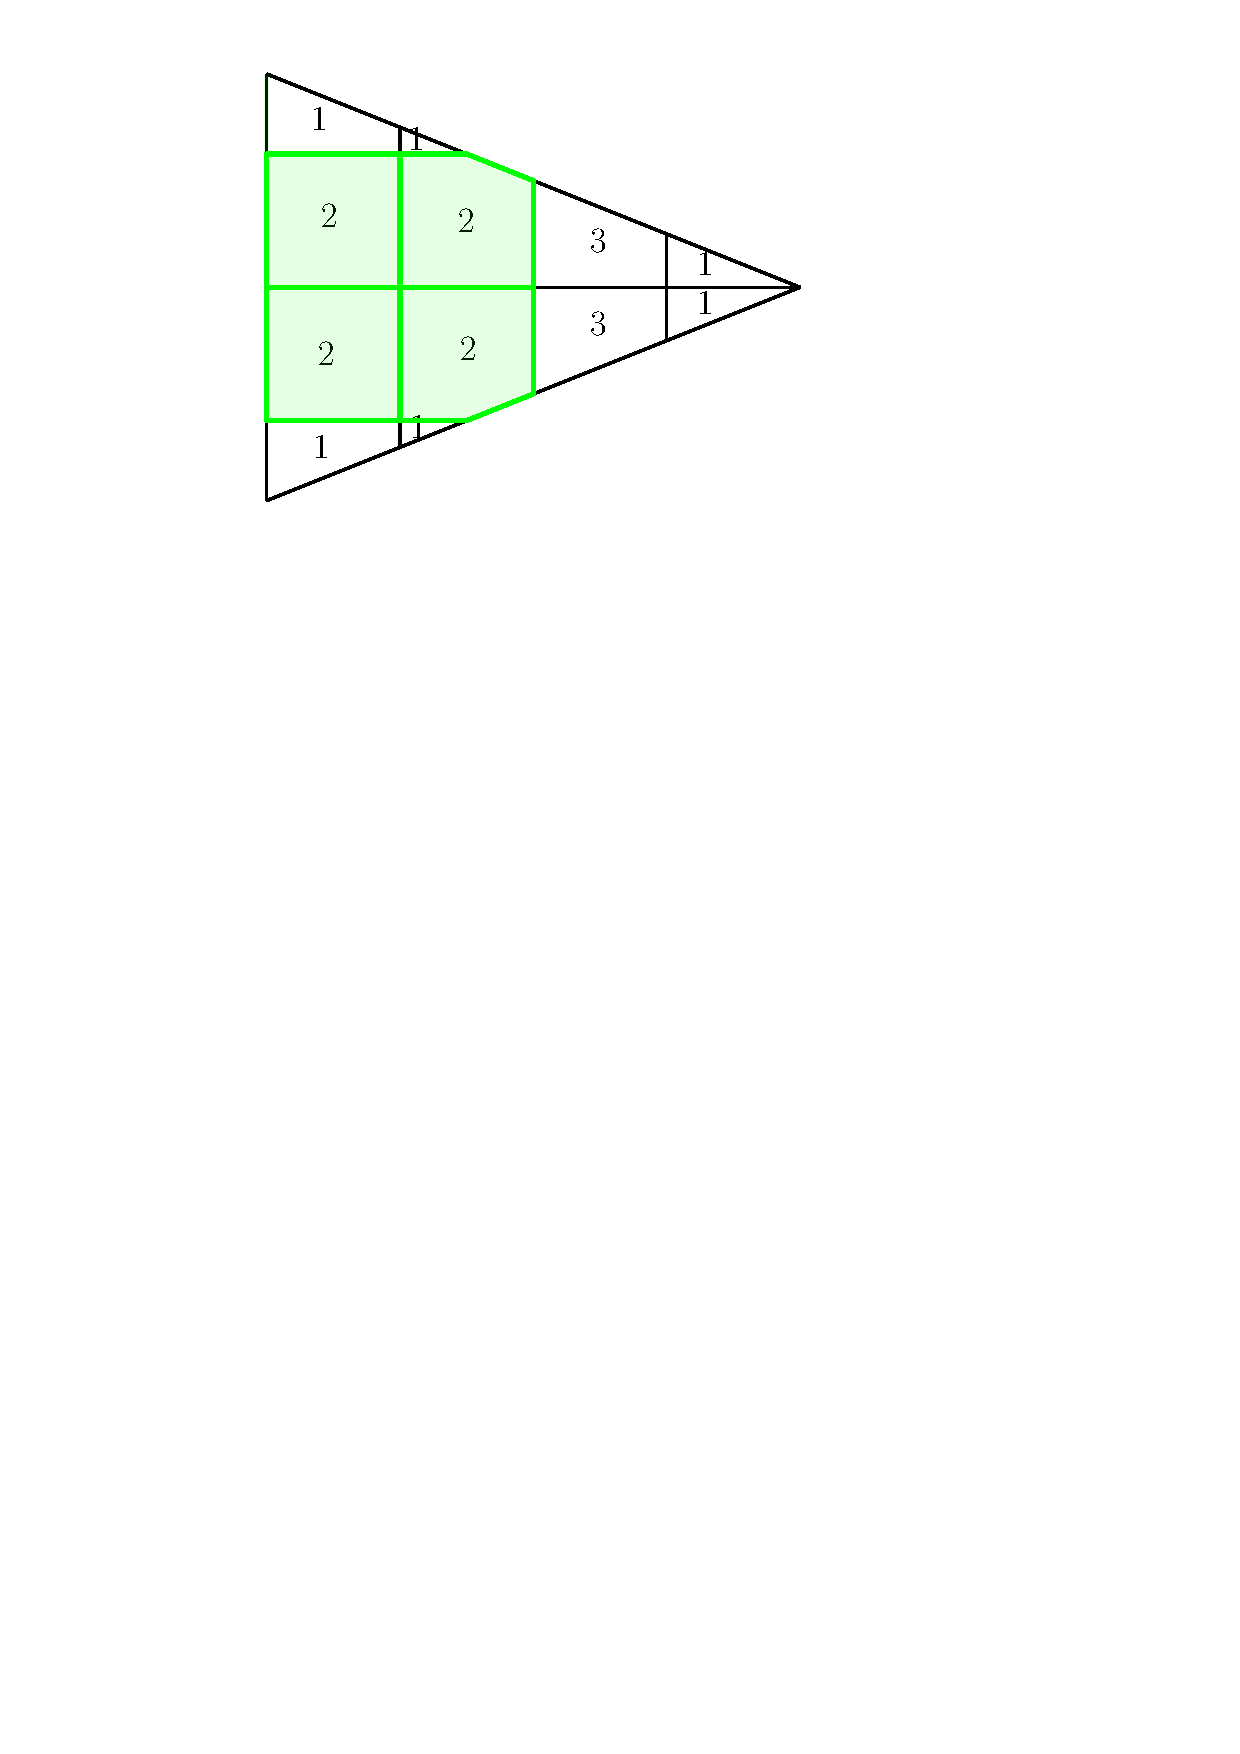
\includegraphics[width=.24\textwidth]{figs/numoverlaps1.pdf} \label{fig:numoverlaps1}}
	\hfill
	\subfloat[]{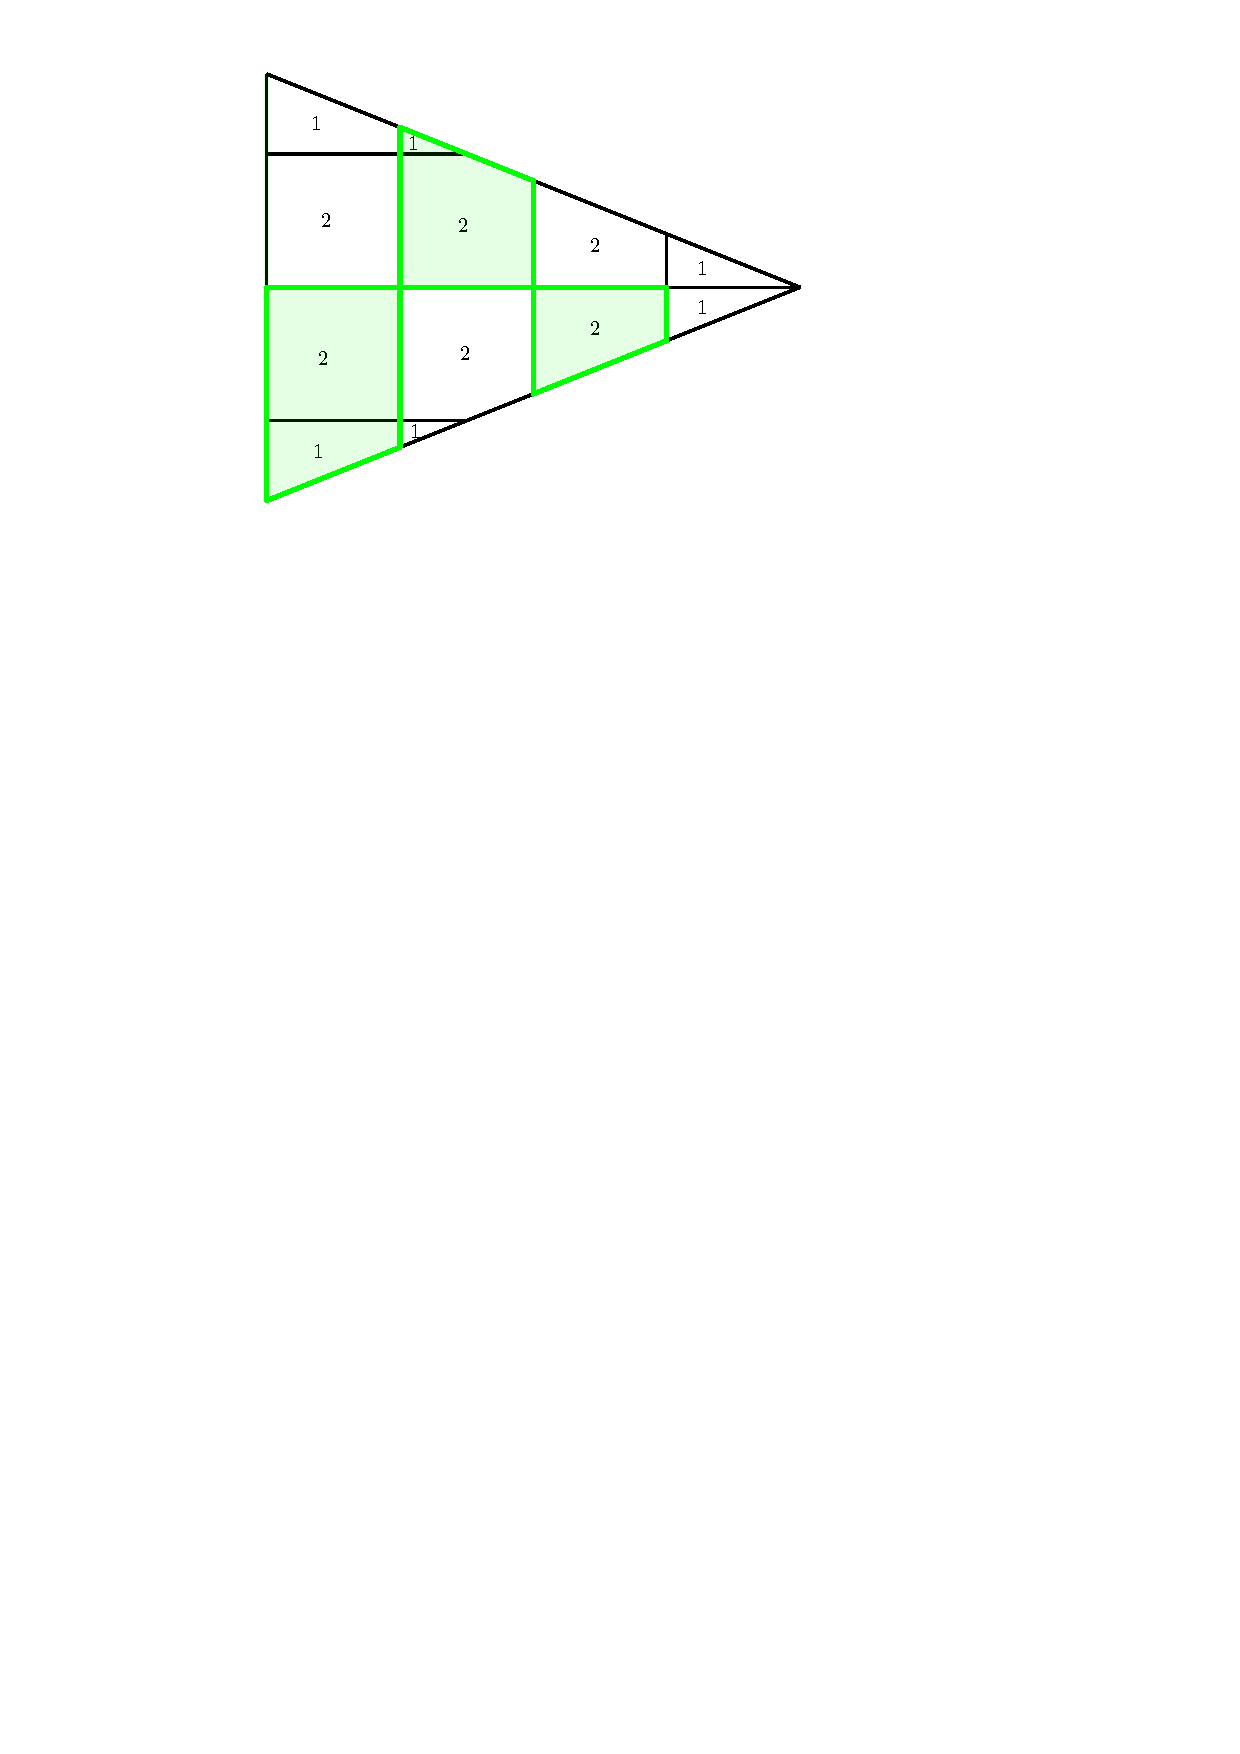
\includegraphics[width=.24\textwidth]{figs/numoverlaps2.pdf} \label{fig:numoverlaps2}}
	\subfloat[]{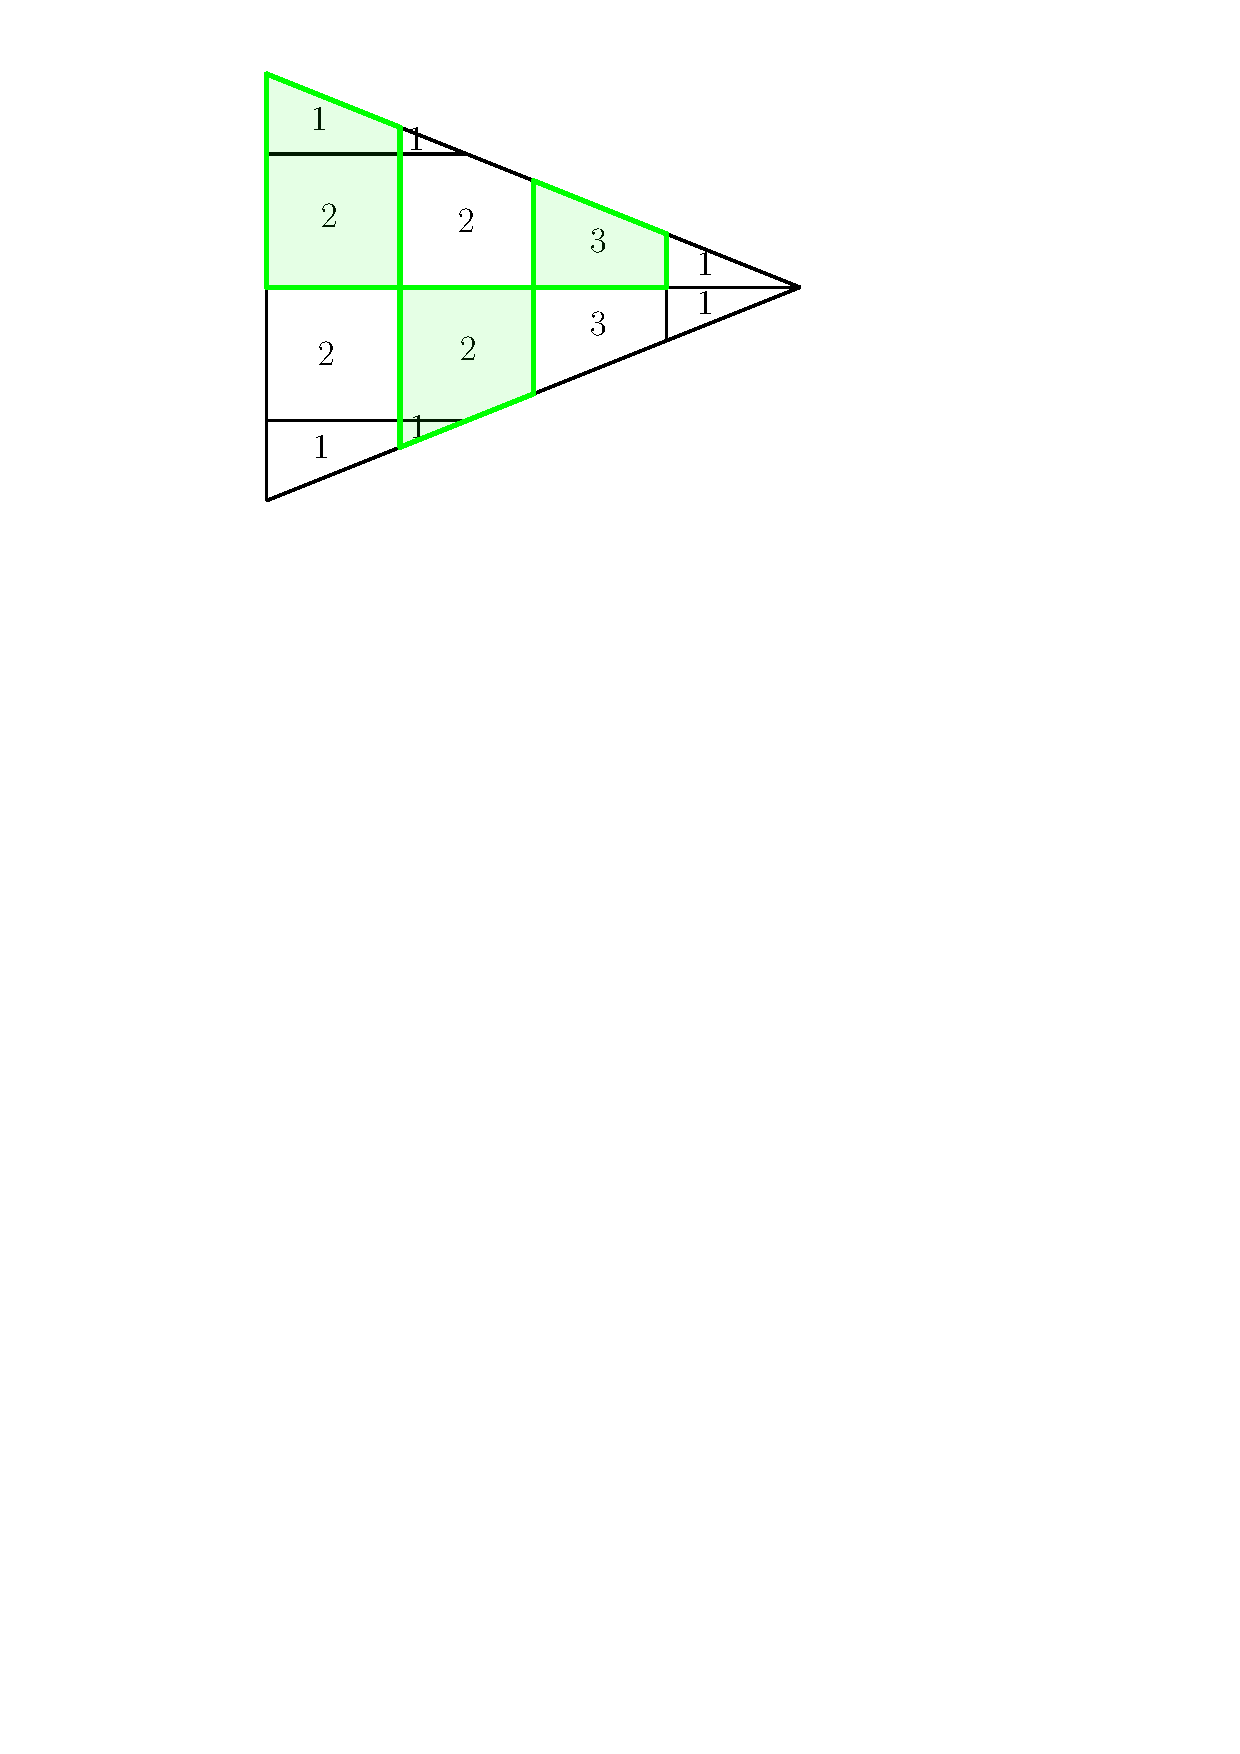
\includegraphics[width=.24\textwidth]{figs/numoverlaps3.pdf} \label{fig:numoverlaps3}}
	\subfloat[]{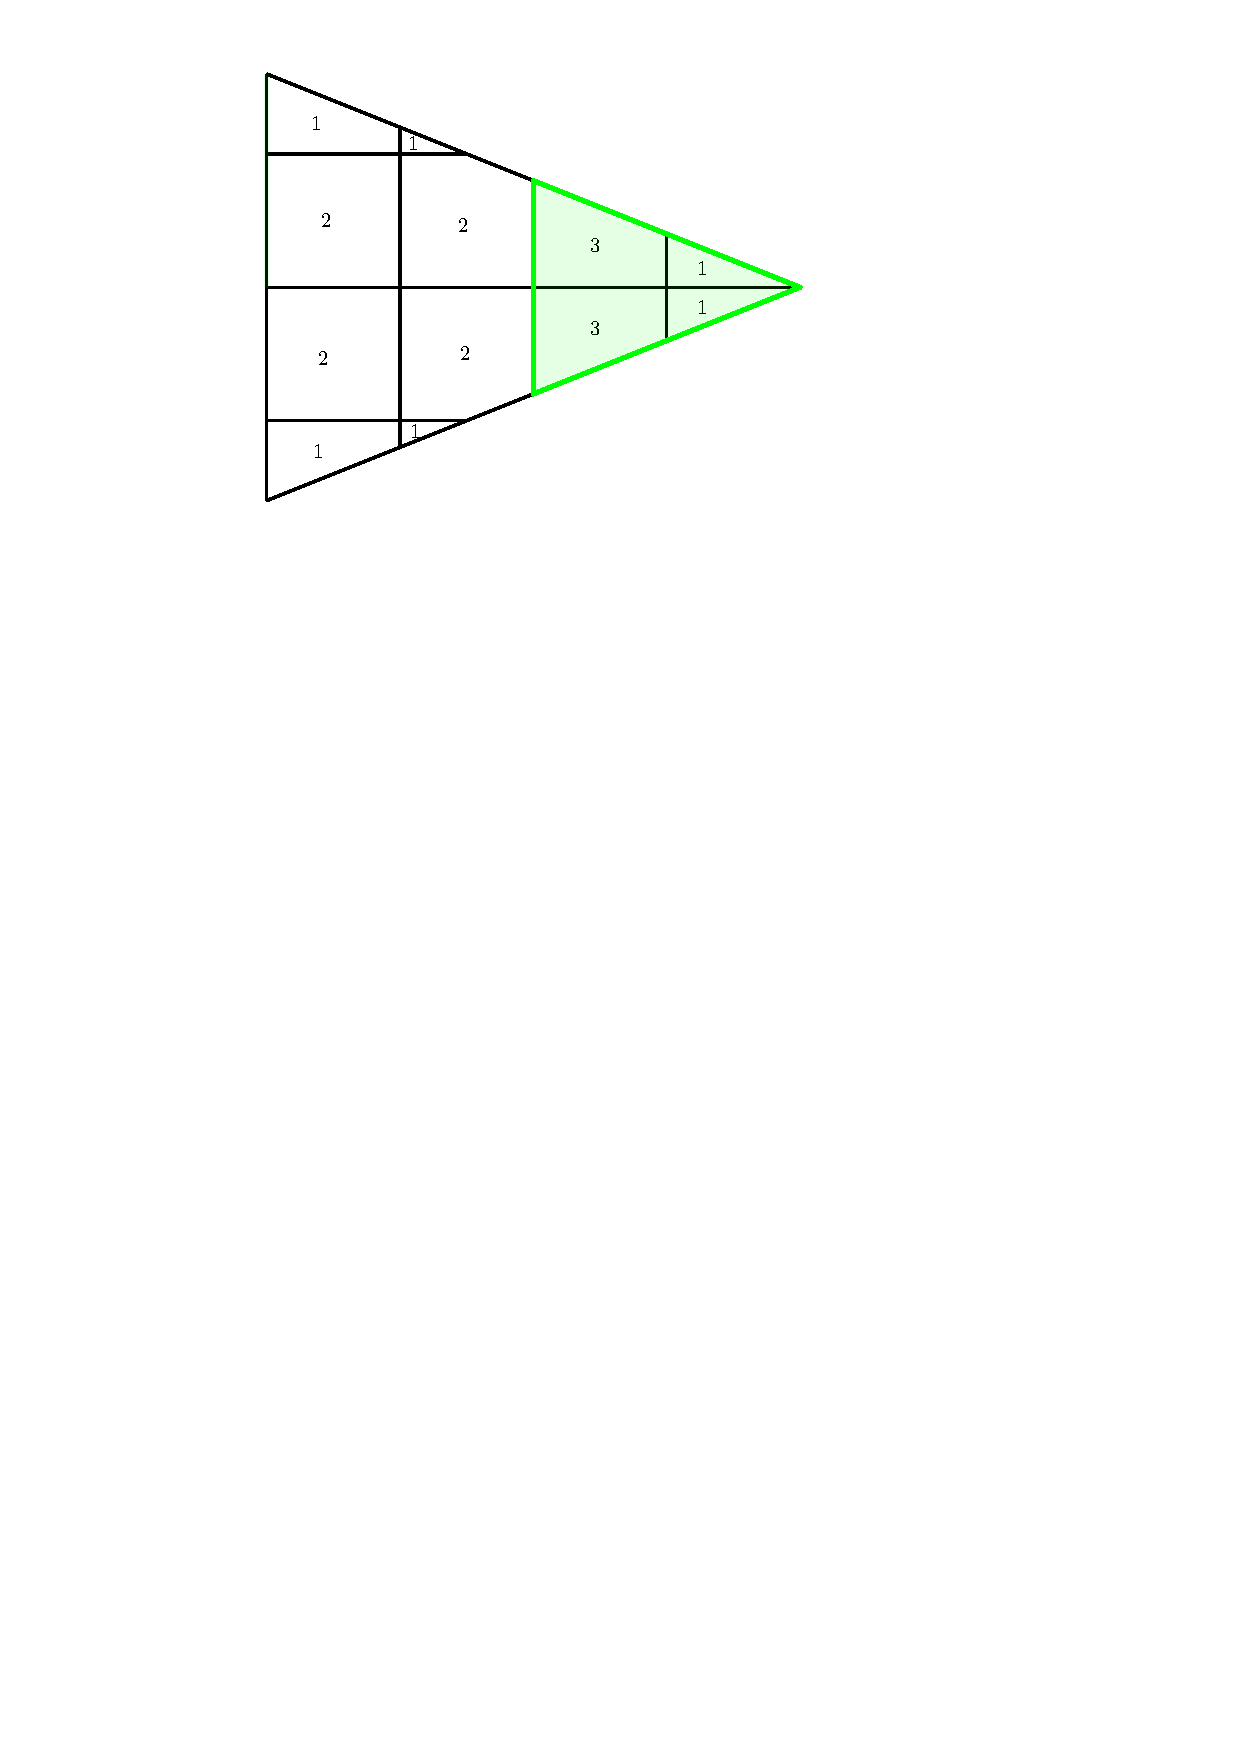
\includegraphics[width=.24\textwidth]{figs/numoverlaps5.pdf} \label{fig:numoverlaps4}}
	\caption{All merging neighborhoods on an example cut cell mesh (in green).  We display the number of overlapping merging neighborhoods on each cell.} \label{fig:overlappingneighs}
\end{figure}
Note that a full cell
can be part of two or more merging tiles if it is placed next to 
several tiny cut cells. An example is shown in
figure \ref{fig:2nborTile}. The cells in green are part of two
neighborhoods, and those in red are part of three.   
 Most full
cells are only members of their own tile and will have a count of one.
Only cells within a narrow band of the cut cells will have a count
larger than one.



\end{itemize}

\begin{figure}[h!]
\begin{center}
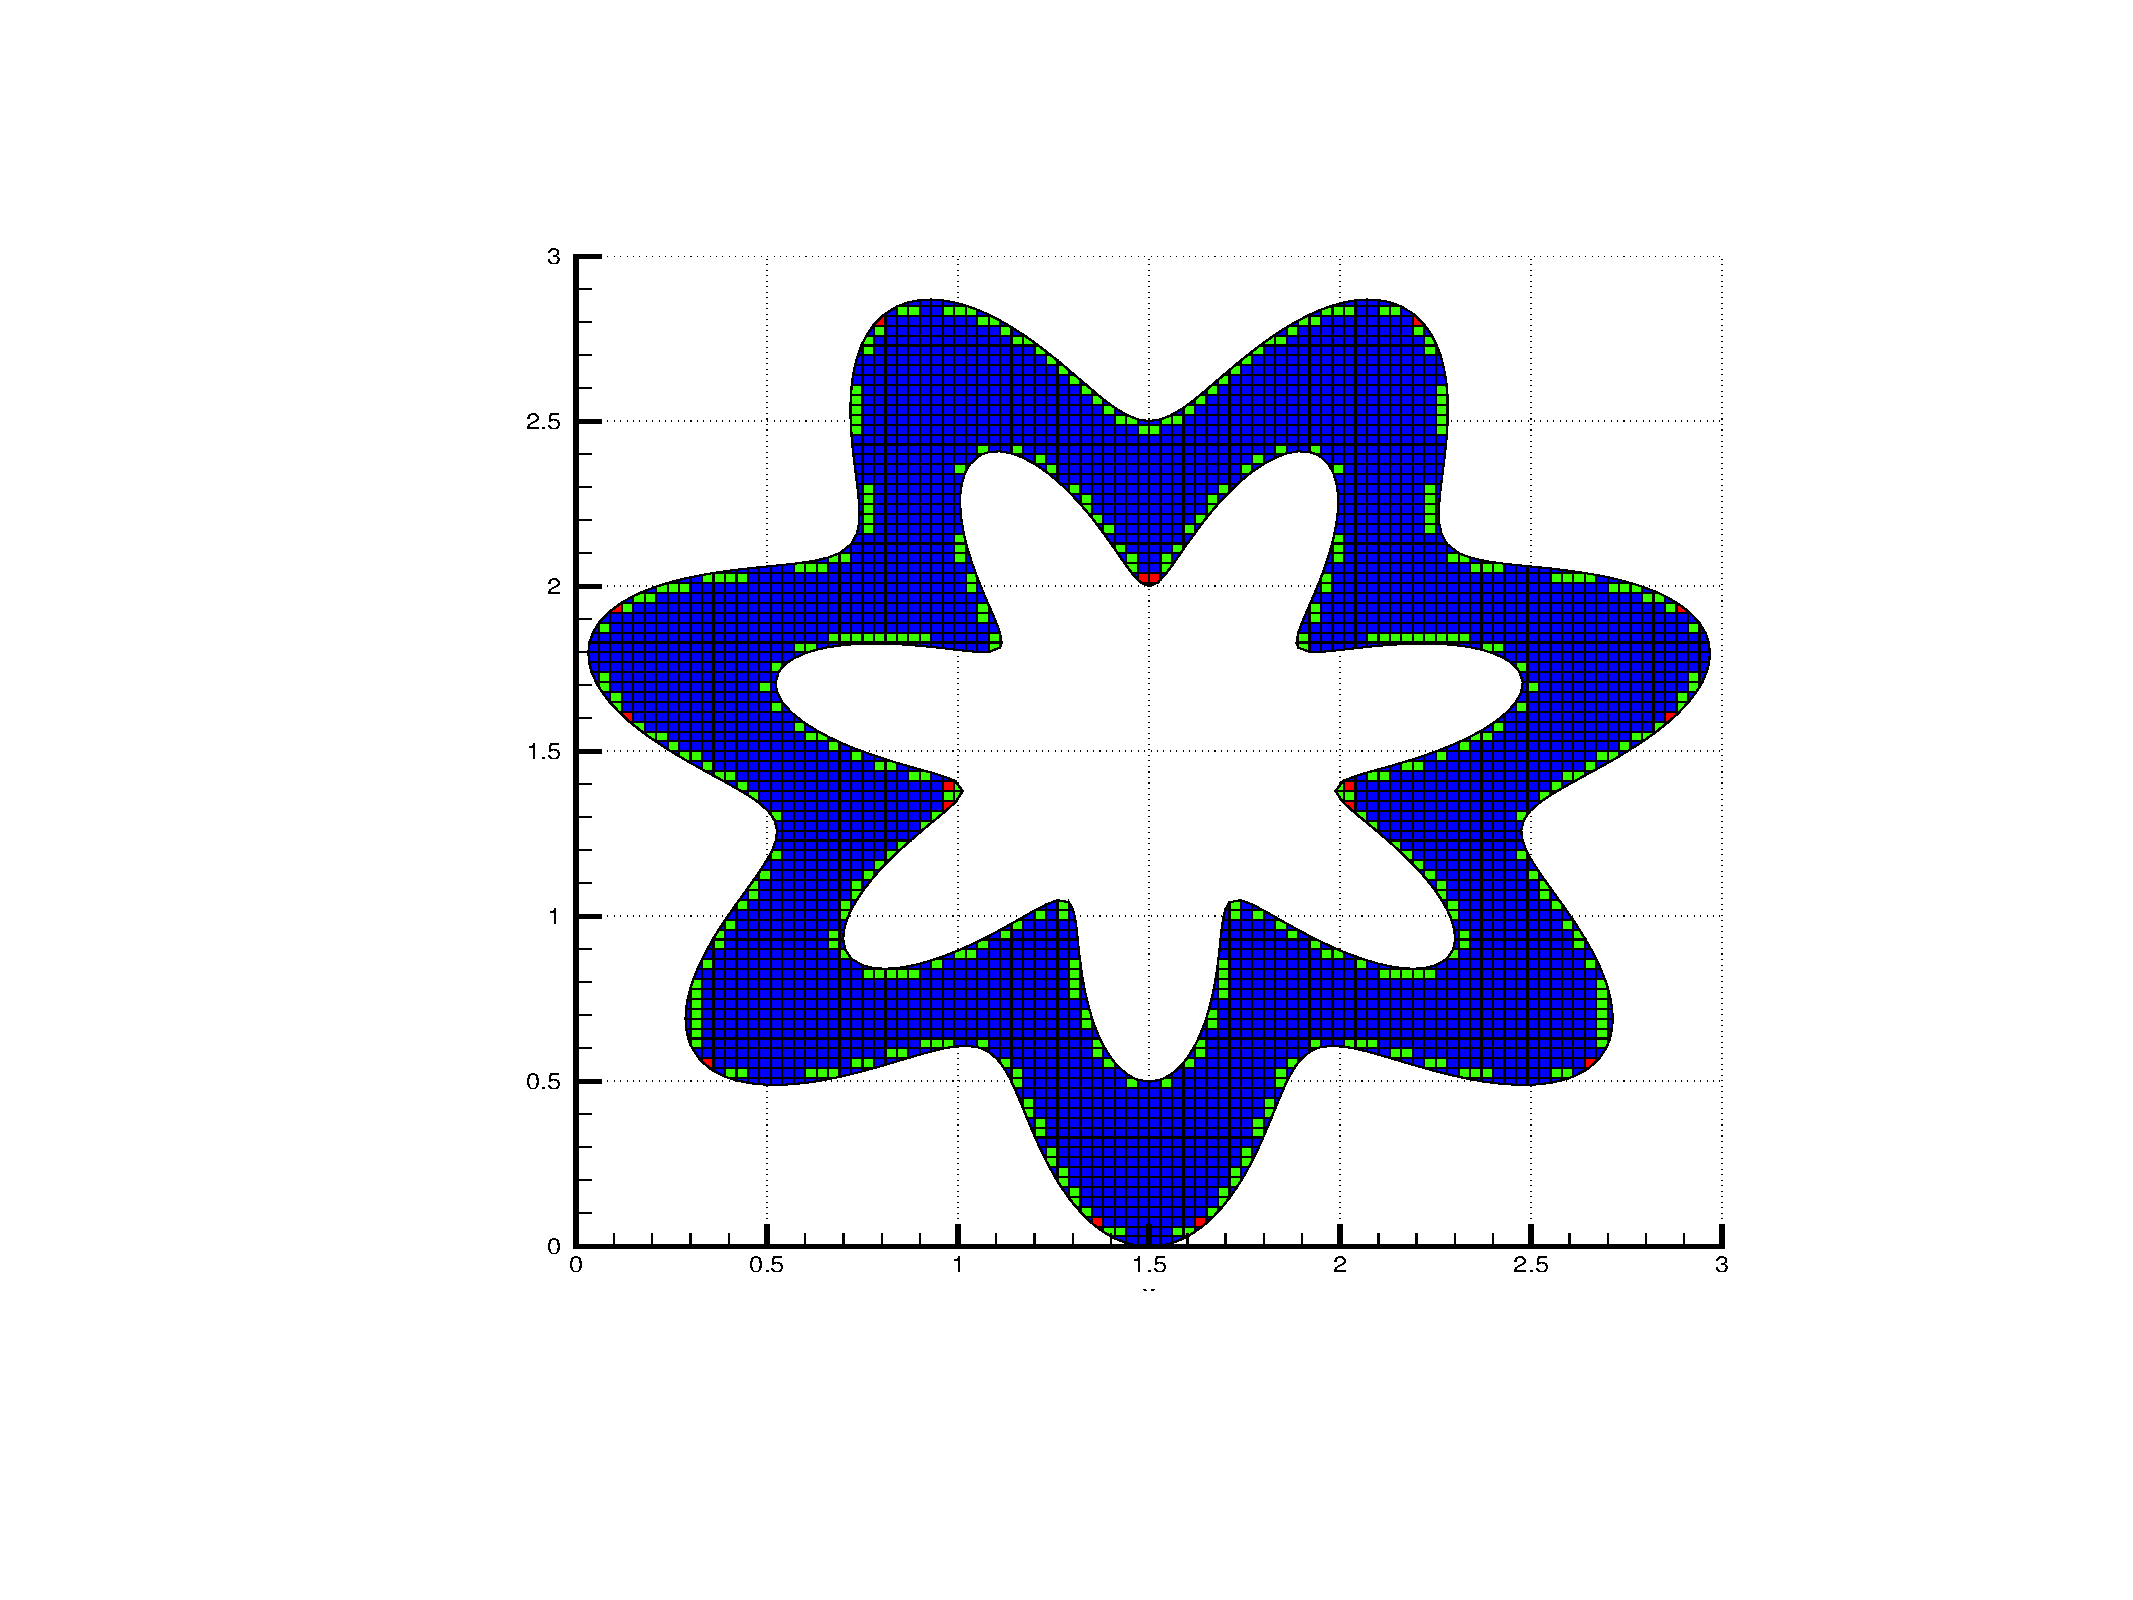
\includegraphics[width=4.1in]{figs/wavyfig.pdf}
\caption{\sf Domain from example XX.  Figure shows how many
neighborhoods each cell belongs to: 
one (blue), 2 (green), or 3 (red).
The full example is shown in section \ref{sec:compResults}.}
\label{fig:2nborTile}
\end{center}
\end{figure}

The two steps above can be part of a preprocessing step, since they do not
depend on the computed solution. For moving geometry however they would
be done at each step.

Using the merging tiles and the cell counts, the state redistribution
algorithm is as follows:

%\begin{enumerate}[label=Step \arabic*:,leftmargin=2\parindent]
\begin{enumerate}
\item
{\bf Compute the volume-weighted and count-weighted solution for all
merged tiles.}   

\vspace*{.1in}
The contribution of each cell is divided by the number of neighborhoods 
it is part of (i.e. its count). The notation in this section refers
to cut cell $i,j$, with solution $U_{i,j}$ and volume
$V_{i,j}$. 
The provisionally update solution before the
stabilization algorithm is applied is $\hat{U}_{ij}$.
There will now be many temporary merging neighborhoods which 
we denote as $\widehat{Q}_{i,j}$. 
Let $M_{ij}$ denote the set of cell indices in the cell $(i,j)$ merging
neighborhood.  Then
\begin{equation}
\label{tiledef}
\widehat{Q}_{i,j} =  \frac{1}{V_m} \, \sum_{k \in M_i} \,  
\frac{V_k}{N_k}  \,\,  \hat{U}_k
\end{equation}
where the volume ${V_m}_{ij}$ is the merging tile volume similarly weighted,
\begin{equation}
\label{voldef}
{V_m}_{ij}  =  \sum_{k \in M_i } \,  \frac{V_k}{N_k}  .
\end{equation}

In other words, the contributions from each cell are weighted by the
number of neighborhoods they contribute to.
In the above equations, $k$ is  a multi-index ranging over the neighbors 
of cell $i,j$ included in its merging tile.
Note that most full cells will have ${V_m}_{ij} = V_{i,j}$, 
and $\widehat{Q}_{ij}  = \bar{U}_{i,j}$.





\item
{\bf Compute a (limited) gradient and weighted centroid for each merging
tile.}

\vspace*{.1in}
For cut cells, a least squares procedure  similar to the one used for
the finite volume update is an obvious choice. However instead of using the
solution $U_{i,j}$ on the Cartesian mesh at time $t_n$,
the merged tile solution  $\widehat{Q}_{i,j}$ is used. It is important
to note that the centroid of the merged tile is NOT the 
centroid of cell ${i,j}$. It could happen, as in figure \ref{fig:
2nborTile} that the centroids are too close to each other to compute a
gradient in the normal direction. If the centroid are not at least
$0.5\,dx$  and $0.5\,dy$ apart in $x$ and $y$ then we increase the
stencil size for the gradient computation TO WHAT. OR DO WE ALWAYS USE a
3by3 NHOOD FOR GRADIENTS?
The same neighborhood that is used for computing the gradient can be
used to limit the gradient to prevent overshoots.
The centroid is computed using the same weighting by number of
neighborhoods as when the volume was computed. (IS THIS TRUE AND IS IT
NECESSARY) NEED DISCUSSION OF NOT A REAL CENTROID

For most full cells with a count of one, the normal gradient
computation as done in the finite volume update will suffice.

\item
{\bf Replace the provisionally computed cut cell values and their adjacent
full cell neighbors with  the contributions from the merged tiles.} 

\vspace*{.1in}
To use the example of figure \ref{fig:2nborTile}, the cut cell value
\begin{equation}
   U_{i,j}^{n+1} := \widehat{Q}_{ij} 
   + (x_m - x_{i,j}) \, \frac{\partial \widehat{Q}_{ij}}{\partial x} 
   + (y_m - y_{i,j}) \, \frac{\partial \widehat{Q}_{ij}}{\partial y}
\end{equation}
since cell ${i,j}$ only belongs to one neighborhood. The adjacent full cell
on the other hand belongs to two neighborhoods -- the one it shares with
the cut cell $i,j$ , and its own merging neighborhood.
So its solution at time $t_{n+1}$  becomes
\begin{equation}
\label{eqn:numhood2ex}
\begin{split}
   U_{i,j+1}^{n+1} \,=\, & \frac{1}{2} \times \left
   (\widehat{Q}_{ij} 
   + (x_m - x_{i,j+1}) \, \frac{\partial \widehat{Q}_{ij}}{\partial x} 
   + (y_m - y_{i,j+1}) \, \frac{\partial \widehat{Q}_{ij}}{\partial y} \right ) \, + \\
    & \frac{1}{2} \times \widehat{Q}_{i,j+1} .
\end{split}
\end{equation}
The last term  in eq. \eqref{eqn:numhood2ex} has no gradient terms because the
centroids of the original cell and merged cell are identical.
The fraction $\frac{1}{2}$ is because cell $(i,j+1)$ is part of  two
neighborhoods, so each contributes half of the solution.

\end{enumerate}

Different choices of neighborhoods, the minimum volume for the merging
neighborhood, gradient neighborhoods, and limiting will give
somewhat different computational results. Some of these will be examined
theoretically using model problems in one space dimension in section
\ref{sec:theory}. These choices can affect the stability limit of the
overall method.
We will also show computational results using different neighborhood
choices in section \ref{sec:compResults} in two space dimensions.

The conservation properties of the algorithm will be discussed after the
higher order SRD algorithm is presented in the next
section (PR PUT IT HERE). It will also be prseented more generally.   
OTHER THINGS HERE? DEMONSTRATE LINEARLY EXACT SECOND ORDER CONVERGENCE
HERE INSTEAD OF COMPRESULTS SECTION?

SOMEHWERE PUT IMPLEMENTATION SUBSECTION OR AT LEAST A PARAGRAPH
TO NOTE THAT THE CELL DOESNT KNOW WHO GIVES TO
IT, SO THIS LOOP IS OVER GIVERS  NOT RECEIVERS.
